\chapter{Algorithm Implementation}
In this chapter, some of the algorithms of the theory chapter are combined, tested and evaluated. The goal is to find the most robust combination of algorithms to detect the pupil, even in a very demanding data set like the LPW. In general, the evaluation can be split up into two parts. 

The first part is the localization of the pupil and the second part is finding the pupil contour estimation. The importance of the localization is that it is possible to create a region of interest (ROI) with the information on the pupil's location. Extracting the ROI has the benefit that the image size is already decreased in the second part, and the computational effort is reduced. 

Important to note is that all algorithms make the basic assumption that the pupil is always visible. Blinking is not counted as a failure and is excluded from the evaluation if possible. For detecting blinking, other algorithms need to be used to preprocess every frame and detect if the eye is closed or not. 


\section{Localization}
For the localization, mainly thresholding, edge detection and haar-like features were implemented and can now be evaluated. The task of a localization algorithm is to extract a ROI that contains the complete pupil. 

\subsection{Thresholding}
 An adaptive algorithm was created to make thresholding more flexible when choosing the best-fitting threshold value $t$. The histogram is used to determine the highest peak in the low-intensity range
\begin{equation}
    t = \text{argmax} \{h(i) | i \in [0,255]\}
\end{equation}
With $h(i)$ being the histogram of the image. The threshold value $t$ is then used to calculate a range for using double thresholding to extract the pupil. The image is modified by setting all values below and above the threshold value to 0. 
\begin{equation}
    f(x,y)= \begin{cases}
        0 &if \quad I(x,y) < t-35 \quad \text{or} \quad I(x,y) > t+25 \\
        I(x,y) &otherwise
    \end{cases}
\end{equation}

Important to highlight is that the peak intensity is not centered in the thresholding range. This assumption derives from testing and can be justified with the probability that a pixel with a lower intensity value than $t$ belongs to the pupil is higher than that of a pixel with higher intensity values than $t$. This approach works well in an environment with almost no noise and no reflections. However, as already mentioned in the theory section, reflections lead to a less high peak in the histogram, and the possibility exists that the threshold value has no peak in the lower value range, leading to a faulty result that can not be used to create a ROI.

The mask created has intensity values between $[t-35, t+25]$. The possibility of creating a binary mask exists and helps create a ROI. To create a ROI all the contours of the binary mask are evaluated on their circularity and the location of the contour with the best circularity and the greatest area will be used as a ROI.
\begin{figure}[h]
    \centering
        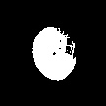
\includegraphics[width=0.3\linewidth]{plots/thresh.png}
    \caption{Thresholding and circularity used to extract ROI}
    \label{fig:threshold_roi}
\end{figure}
In an environment with nearly no noise, this method works flawlessly and almost in real-time. Thresholding is keen to struggle with noise and is therefore not useful for the LPW data set.
\subsection{Edge detection}
Edge detection is strongly affected by noise, and therefore preprocessing is vital for valuable results. Every frame undergoes the same preprocessing as in the other algorithms, but a Gaussian blur is used additionally to weaken small fast-changing intensity regions that can be considered noise.

Even though Gaussian blur is used, pupil contour information is still missing because the contour is covered by noise and can not be recovered. The edges are detected, but the same problem as with thresholding arises here. By using Sobel and then the Canny edge detection, the results are useful in an environment with almost no noise. Canny edge detection needs two threshold parameters to work correctly and also here arises the problem that these parameters need to be adaptive to the environment, which can be tricky. 
\begin{figure}[h]
    \centering
        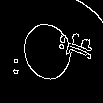
\includegraphics[width=0.3\linewidth]{plots/edge_detection.png}
    \caption{Edge Detection used to extract ROI}
    \label{fig:edge_roi}
\end{figure}

\subsection{Haar-like feature detection}
The Haar-like feature detection is the approach that is proposed by this thesis to find the region of interest. It has the best detection rate of all approaches tested on the LPW data set and is therefore the best approach to finding the ROI. The Haar-like feature is constructed as described in the theory part and is shown in \ref{fig:haar_features}. 
The calculation of the response matrix is done by using the integral image and is calculated multiple times with variating radius $r$. All response matrixes are compared, and the location of the highest response is returned as a point that can be considered to be inside the pupil. 

\begin{figure}[h]
    \centering
    \begin{subfigure}{0.5\textwidth}
        \centering
        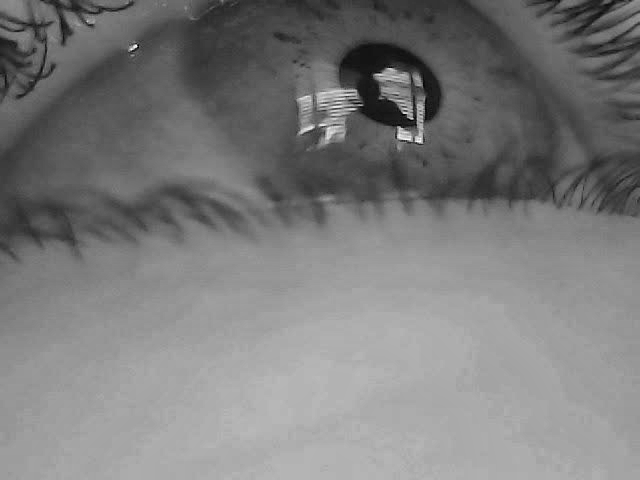
\includegraphics[width=0.9\linewidth]{plots/results/originalbest.png}
        \caption{Original Frame}
    \end{subfigure}%
    \hfill
    \begin{subfigure}{0.5\textwidth}
        \centering
        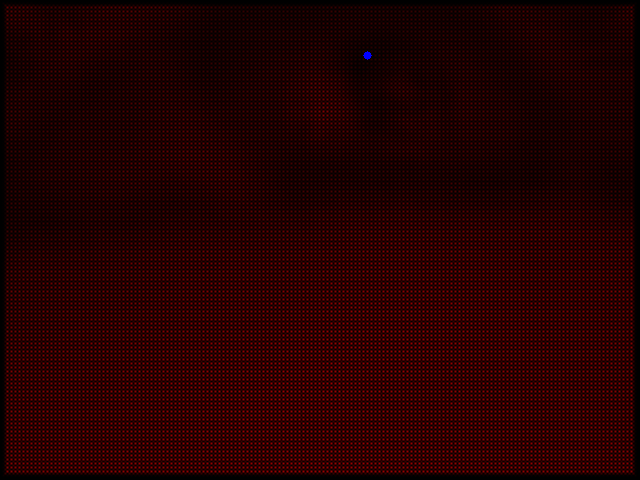
\includegraphics[width=0.9\linewidth]{plots/results/responsehaarbest.png}
        \caption{Response matrix, blue is the best response}
    \end{subfigure}%
 
    \caption{Response Matrix for pupil detection}
    \label{fig:limit_haar_good}
\end{figure}

The strongest response lies within the pupil, and the location is used to create a ROI. In this case, a ROI of $(220 x 220)$ was the norm size, but depending on the rescaling of the video, this needs to be adapted. Important to note is that the returned point in the pupil is not given to be in the center, and this in an important fact when choosing the size of the ROI.
Nevertheless, Haar-like feature detection still needs improvement and even though it can handle noise, there are limits to the amount of noise until the algorithm fails. Furthermore, the algorithm is not able to detect the pupil when the eye is closed.

\begin{figure}[h]
    \centering
    \begin{subfigure}{0.5\textwidth}
        \centering
        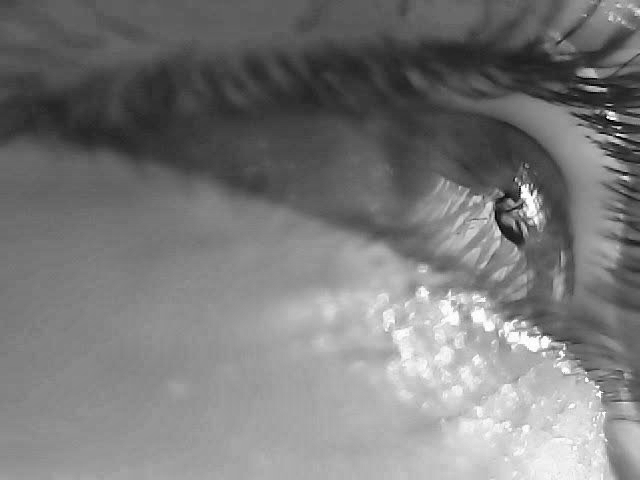
\includegraphics[width=0.9\linewidth]{plots/results/originalworst.png}
        \caption{Extreme noise example}
    \end{subfigure}%
    \hfill
    \begin{subfigure}{0.5\textwidth}
        \centering
        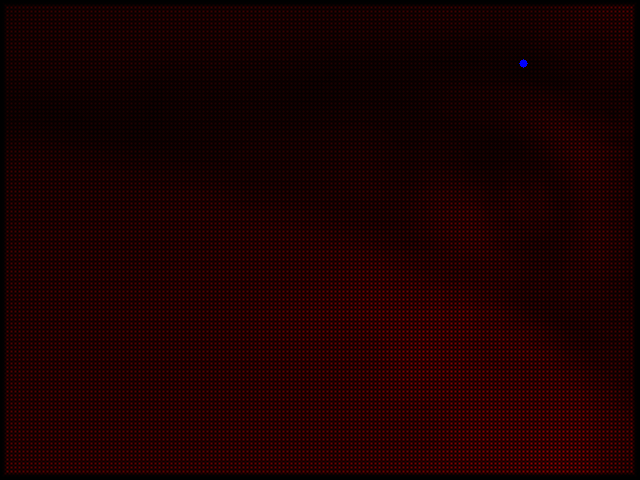
\includegraphics[width=0.9\linewidth]{plots/results/responsehaarworst.png}
        \caption{Response Matrix result with best response}
    \end{subfigure}%
 
    \caption{Limits to the Haar-like feature approach}
    \label{fig:limit_haar}
\end{figure}
The problem with the LPW data set is that it is so versatile and the conditions change during the recording. Therefore, finding an approach that can adapt to all the conditions and perform well in a given time interval is hard. Of all the localization algorithms Haar-like feature outperformed every single one and is the most adaptable to changing environmental conditions and different eye positions. The performance of the Haar-like feature detection was improved by using the ThreadPool Executor from the concurrent.futures library and from numba the njit library.

ThreadPool Executor makes it possible to use multithreading and njit compiles the sliding window over the integral image and the calculation of the response matrix for the Haar-like feature to machine code. The use of those two libraries makes the algorithm run about ten times faster. 

\section{Ellipse parameter estimation}
In the second part of pupil detection, it is necessary to make use of the location information from the first part and build on this foundation to find the five ellipse parameters: center: $(x,y)$, axis: (major, minor) and angle. The LPW has labels for the center only of the pupil, and therefore only the center can be used to evaluate the performance of the algorithms. A second evaluation has to be done manually by inspecting the fit of the ellipse to the pupil contour. This is hard to evaluate with numerical methods and the results must therefore be taken with a grain of salt. In this section four different algorithms will be discussed and evaluated: The OpenCV ellipse fit based on contours (binary thresholding), Canny edge detection with OpenCV Ellipse fit,  ACWE with OpenCV Ellipse fit, and ACWE combined with RANSAC.

\subsection{Thresholding and OpenCV ellipse fit}
\label{sus:thresholding_ellipse_fit}
The benefit of this method is that it can run in real-time and still perform well in specific frames when the noise amount is low, and the pupil is completely visible. However, as mentioned in the localization part, this combination is not robust enough to handle the LPW data set. The thresholding is done with the same approach as in the localization part and the binary mask is then used to find the contours. The contours are then evaluated by their circularity and the similarity to an ellipse. The contour with the biggest area is further used with the OpenCV ellipse fit function. 

The OpenCV ellipse fit function is based on the least square method and is robust and fast. The problem with the least square method for ellipse fitting is that the method tries to find an ellipse that minimizes the distance from every point on the boundary of the binary mask to the ellipse curve. When the pupil is partially covered by noise, the contour can not match the original shape of the pupil and is not the total pupil boundary. Using the least square method leads to a faulty ellipse fit where the result is not usable. The amount of outliers is too high, and the ellipse fit is not accurate enough because there is information missing. The problem can be seen in the visualization of the OpenCV ellipse fit:
\begin{figure}[h]
    \centering
    \begin{subfigure}{0.3\textwidth}
        \centering
        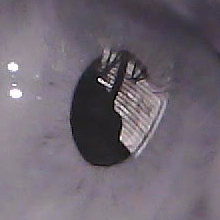
\includegraphics[width=0.9\linewidth]{plots/results/roi_text_resutls.png}
        \caption{ROI}
    \end{subfigure}%
    \hfill
    \begin{subfigure}{0.3\textwidth}
        \centering
        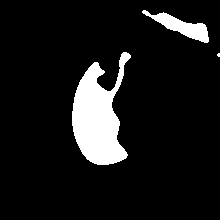
\includegraphics[width=0.9\linewidth]{plots/results/roi_binary_ellipse.png}
        \caption{Binary thresholding}
    \end{subfigure}%
    \hfill
    \begin{subfigure}{0.3\textwidth}
        \centering
        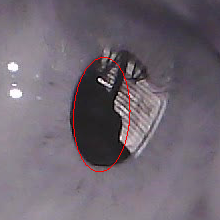
\includegraphics[width=0.9\linewidth]{plots/results/roi_result_binary_ellipse.png}
        \caption{OpenCV Ellipse fit}
    \end{subfigure}%
    \caption{Binary thresholding with OpenCV ellipse fit}
    \label{fig:binary_threshold_ellipse_fit}
\end{figure}

\subsection{Canny edge detection with OpenCV ellipse fit or RANSAC}
For this combination, the first step is to find the ROI. This is done with the Haar-like feature. This is from great importance because otherwise, there is no chance of finding the pupil boundary because there will be many edges that are possible pupil edges. The image is blurred with a Gaussian blur. Afterward, the Canny edge detection is used on the ROI (Using the gradient, by calculating the sobel gradient). 

The edges are evaluated by their circularity. The best matching contour is further processed with the OpenCV ellipse fit or the RANSAC alrogithm. This results in the pupil ellipse approximation. The problem with this approach is that the boundary must be clearly visible and the threshold values must be chosen carefully. Here the already known intensity value from the given point inside the pupil is used to make a decision for the thresholding values needed by the Canny edge detection. The benefit of this algorithm is the speed at which the frames can be processed. However, this combination is not considered to be robust enough to handle the LPW data set and is therefore not further evaluated.

\subsection{ACWE with OpenCV ellipse fit}
This approach uses the OpenCV ellipse fit to interpret the results from the ACWE, the benefit is that it runs faster than the RANSAC but it is strongly dependent on the quality of the binary mask returned by the ACWE. If the mask is not completely on the total boundary of the pupil, the ellipse fit will also not fit the pupil because of the least square fit used in OpenCV ellipse fit. 

ACWE and OpenCV ellipse fit also only work in low noise environments, just as the thresholding approach and the Canny edge detection. When comparing the threshold and contour segmentation with the ACWE with OpenCV ellipse fit, it can be seen that the quality of the approximation is almost the same. Nevertheless, in terms of speed, ACWE with OpenCV ellipse fit is decently slower than the thresholding approach. Especially when the pupil is large, the ACWE takes a long time to converge to the boundary of the pupil because the level set $u$ of the ACWE can only grow for a certain amount each iteration. In contrast, thresholding finds the contour of the pupil in a few iterations and in a fraction of the time compared to ACWE.


\subsection{ACWE combined with RANSAC}
\label{sus:acwe_ransac}
The benefit of using ACWE discussed in section \ref{sus:acwe}and the RANSAC method already discussed in section \ref{sus:ransac} is that the ellipse fit is not anymore based on the least square method but instead uses a different approach as already introduced in the RANSAC section. The RANSAC algorithm leads to a better fit but with the tradeoff of computational efficiency. This tradeoff is worth it when the images contain much noise and the pupil boundary is not completely visible. If only a part of the boundary is visible, the accuracy of the ACWE combined with RANSAC is more significant than when just using the OpenCV Ellipse fit.

Haar-like feature detection returns a point inside the pupil. This location is the center position for the initial contour creating the level set $u$. When ACWE converges, the binary mask is dilated and eroded to remove small noise pixels and to make the mask smother. Then the mask is used as input for the RANSAC algorithm to fit an ellipse to the contour of the mask. The parameter of the approximated pupil contour can be retrieved from the ellipse fit.

As already foreshadowed, the process contains many steps and ACWE and RANSAC are iterative algorithms, making this approach the slowest but most accurate of all discussed algorithms and their combination. The RANSAC algorithm uses a subset of five points and fits an ellipse to these points. To evaluate the ellipse fit, the distance from all points of the mask's contour to the ellipse curve is calculated and categorized. The fit is then calculated with these equations: 
\begin{gather}
    \text{InlierRatio} = \frac{n_{\text{inliers}}}{n_{\text{total\_points}}} \\
    \text{BorderRatio} = \frac{n_{\text{border}}}{n_{\text{total\_points}}} \\
    \text{Area} = \pi \cdot a \cdot b \\
    \text{Fit} = \alpha \cdot \text{InlierRatio} + \beta \cdot \text{BorderRatio} - \frac{\text{Area}}{n_{\text{total\_points}}} \cdot \pi
\end{gather}

with $\alpha = 150$, $\beta = 200$, $a$ and $b$ are the major and minor aixs of the ellipse. The $InlierRatio$ is the ratio of inliers to the total number of points, the $BorderRatio$ is the ratio of points on the border of the ellipse to the total number of points and the area is the area of the ellipse. The Fit is then calculated by a weighted sum of the $InlierRatio$, $BorderRatio$ and the $Area$. The weights are chosen by testing and are not optimal but work well enough and can be further adapted. 

In each iteration of the RANSAC the fit is calculated, and if the current ellipse parameters have a greater fit score than all the previous ellipse parameters, the current ellipse parameters are saved as the best fit. After $N$ iterations, the best fit is returned as the approximation of the pupil ellipse. 

The reason for using a fit equation is that the individual conditions can exclude each other. When using conditional logic, the evaluation of a fit becomes tricky and strongly dependent on the order of the ellipses generated. For example, suppose the ellipse has a small area, which is considered a good fit, but only $20\%$ of inliers. In that case, the conditional logic rejects all following ellipses based on the smaller area. Therefore conditional logic is not considered for the evaluation of the ellipses. 
Here are an example fits in a very noisy environments to show the robustness of the algorithm: 
\begin{figure}[h]
    \centering
    \begin{subfigure}{0.4\textwidth}
        \centering
        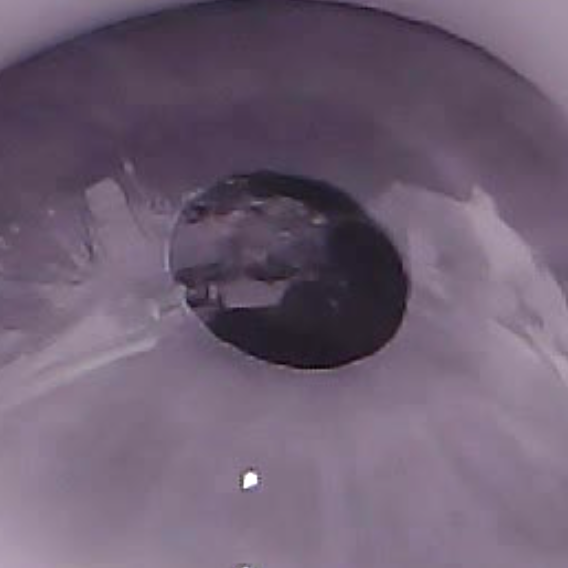
\includegraphics[width=0.9\linewidth]{plots/acwe/robusfit.png} 
    \end{subfigure}
    \begin{subfigure}{0.4\textwidth}
        \centering
        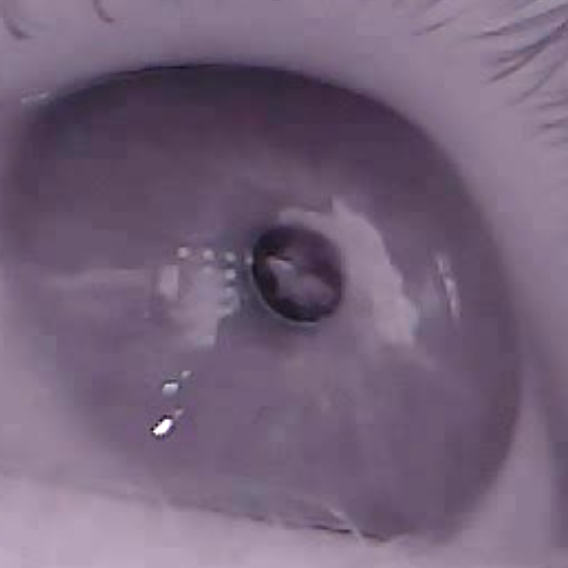
\includegraphics[width=0.9\linewidth]{plots/acwe/robusfit2.png} 
    \end{subfigure}
    \begin{subfigure}{0.4\textwidth}
        \centering
        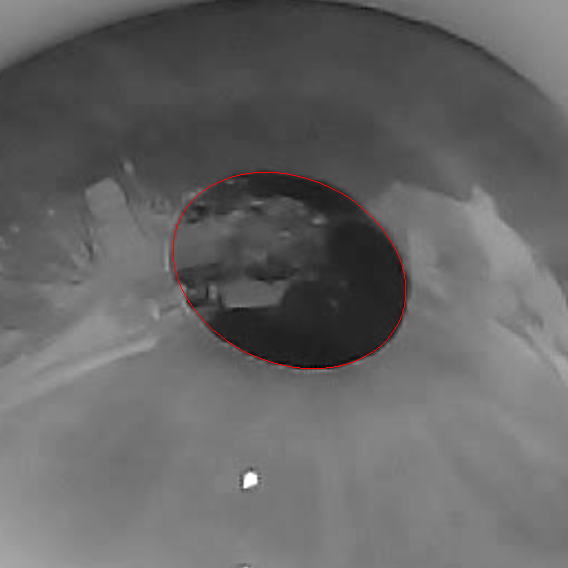
\includegraphics[width=0.9\linewidth]{plots/acwe/robustfitfit.png} 
    \end{subfigure}
    \begin{subfigure}{0.4\textwidth}
        \centering
        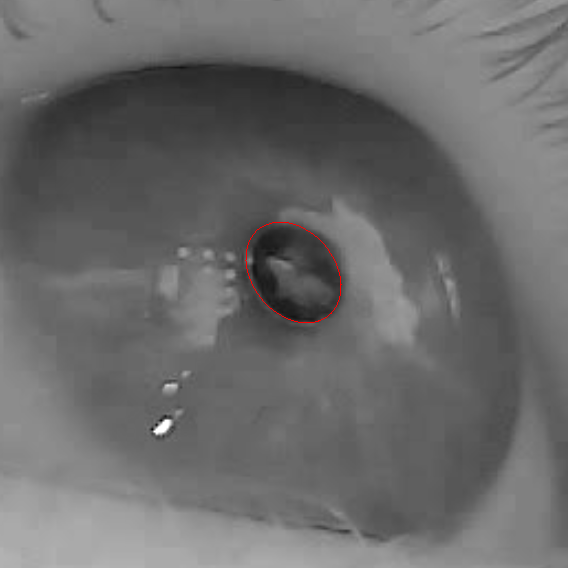
\includegraphics[width=0.9\linewidth]{plots/acwe/robustfitfit2.png} 
    \end{subfigure}
\caption{Example frames with the corresponding pupil approximation}
\label{fig:robust_fit_acwe_ransac}
\end{figure}

